\documentclass[border=10pt]{standalone}
\usepackage{tkz-fct}
\usepackage{tkz-base}
\usepackage{array}

\begin{document}

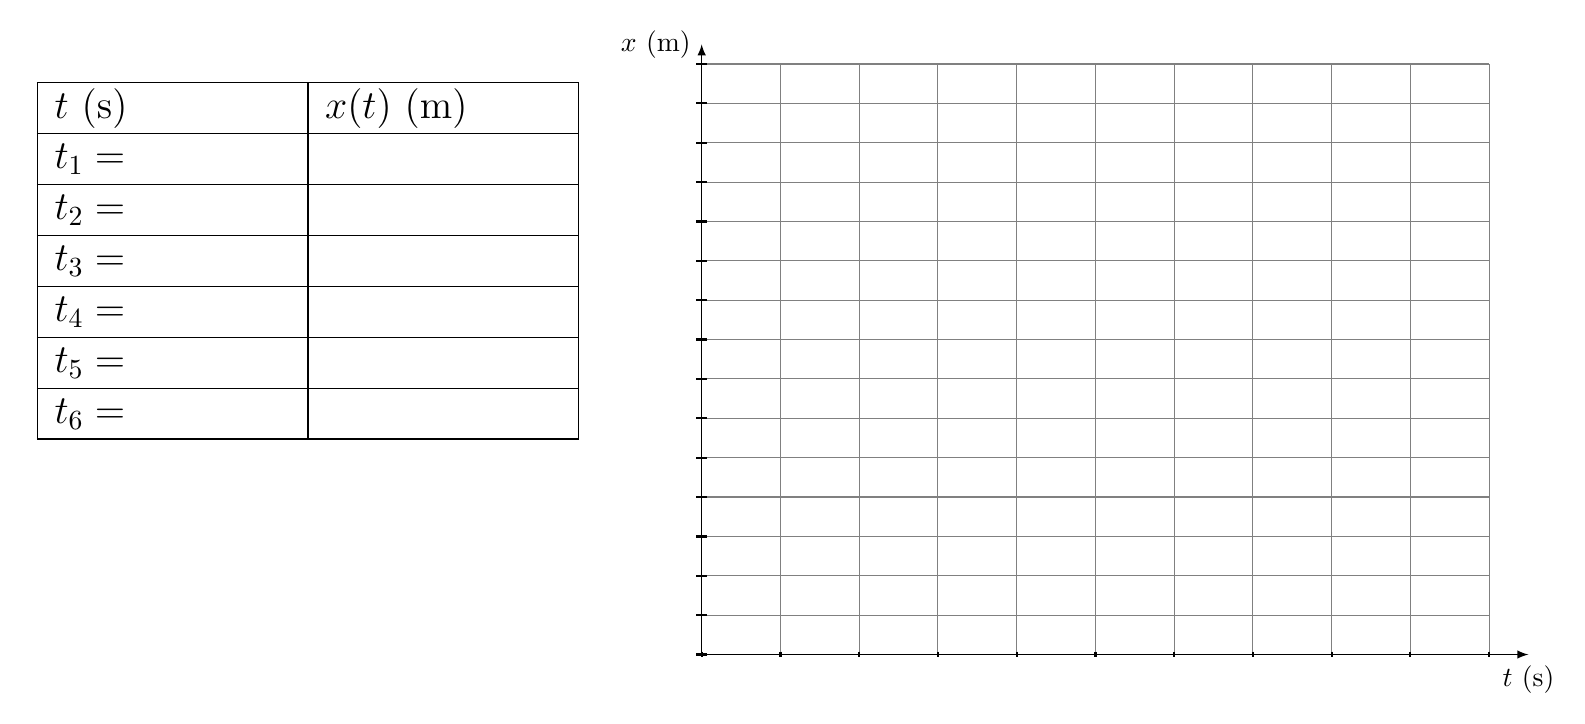
\begin{tikzpicture}
% Tableau en LaTeX standard avec tkz-text
\tkzText(-5,5){\Large
    \begin{tabular}{|p{3cm}|p{3cm}|}
        \hline
        $t$ (s) & $x(t)$ (m) \\
        \hline
        $t_{1}=$& \\
        \hline
        $t_{2}=$& \\
        \hline
        $t_{3}=$& \\
        \hline
        $t_{4}=$& \\
        \hline
        $t_{5}=$& \\
        \hline
       $t_{6}=$ & \\
        \hline
    \end{tabular}
}

% Repère quadrillé
\begin{scope}[yscale=0.5]
\tkzInit[xmin=0,xmax=10,ymin=0,ymax=150, ystep=10]
\tkzGrid
\tkzDrawX[label = $t$ (s)]
\tkzDrawY[label = $x$ (m)]

\end{scope}
\end{tikzpicture}

\end{document}
